\documentclass[twocolumn]{article}
\usepackage{graphicx}
\usepackage{float}
\usepackage{lipsum}

\title{Enhancing household survey microdata accuracy using machine learning: project plan}
\date{}
\author{Nikhil Woodruff}

\begin{document}

\maketitle

\section{Project outline}

Tax-benefit policy is the set of rules that determine tax liabilities and benefit entitlements, deciding the allocation of nearly half of GDP in the United Kingdom alone. When policymakers, think-tanks or academic institutions propose changes to tax-benefit policy, they often use mathematical models to estimate the impact of such changes. The dominant approach to modelling tax-benefit policy is \emph{microsimulation}, a method composed of two parts: a model of policy logic that can compute taxes and benefits for a given household under current and proposed changes, and dataset representative of a target population, on which the policy model is executed. Most microsimulation models use a household survey dataset as their input. The most common of these surveys is the Family Resources Survey (FRS).

The accuracy of microsimulation models is crucial to their utility, and since policy logic is straightforward to verify (since the logic is specified explicitly in legislation), most microsimulation inaccuracy is due to the accuracy of the data. This project will center around the question of \emph{how much can computational methods improve the accuracy of household survey microdata}, predicated on three assumptions which can each be tested: that the unadjusted UK household survey data has poor accuracy for some questions (usually involving low or high income households), that existing methods to improve it distort the data (reducing its accuracy in some areas), and that machine learning-based approaches can significantly improve accuracy across most uses of the dataset. \emph{Accuracy} is not a particularly well-defined term, but here I use the common definition: a household survey's accuracy is the extent to which it gives answers to questions that are close to questions posed directly to the target population.

Broadly, the main problems with the FRS are that we know it is inaccurate for at least two groups: high incomes and benefit claimants - we know this because more robust surveys (administrative datasets) give substantially different answers to questions (for example, total budgetary imapcts of programs). Common methods are largely unchanged over the past few decades, often limited to percentile-based logic or nearest-match imputation. Machine learning methods have become transformative in many other fields as a way of learning complex data relationships, but they are largely unexplored in the context of public policy analysis. Specifically, this project will benchmark a new pipeline based on two machine learning techniques to maximise survey accuracy: gradient descent to determine optimal data weights (counteracting sampling bias) and random forest model imputation to edit data values (counteracting measurement error in particular variables). These are two methods for which there is a wealth of evidence of efficacy and robustness, and their agnostic nature (they are not designed with any assumptions about the data context) will serve to assess any weakness in the current approaches, which use explicit data assumptions.

In order to assess these improvement methods, this project will create a computational method of estimating survey accuracy, which aggregates as many known sources of truth as possible (e.g. from census data and administrative statistics) and measures a survey dataset's deviation from each of these data. I will then implement both machine learning models, applying them together to minimise this loss function, and assess the change in accuracy over the original surveys.
\section{Project plan}

Each task, numbered below, is shown in the Gantt chart in Figure \ref{gantt_chart}. Each task is labelled with its importance, from highest to lowest: basic (B), intermediate (I) or advanced (A).

\begin{enumerate}
    \item \textbf{Literature review} - review the literature on survey accuracy, survey improvement techniques, and machine learning methods for survey improvement. (B)
    \item \textbf{Implement percentile adjustment} - implement a method of percentile adjustment in Python. (B)
    \begin{enumerate}
        \item Implement both original SPI and SPI2 algorithms used by the ONS. (I)
        \item Research and implement exact algorithms used by other UK think-tanks. (A)
    \end{enumerate}
    \item \textbf{Implement percentile adjustment} - implement a method of percentile adjustment in Python. (B)
    \item \textbf{Implement record matching} - implement a method of record matching in Python between the FRS and Survey of Personal Incomes (HMRC administrative data). (B)
    \item \textbf{Implement survey accuracy estimation} - implement the accuracy estimation function for the FRS, using UK administrative data points. (B)
    \begin{enumerate}
        \item Compare the accuracies of the FRS and other household surveys under this new loss function, to establish the relative accuracy of the baseline survey. (I)
    \end{enumerate}
    \item \textbf{Implement gradient descent-based reweighting} - implement gradient descend-based reweighting in Python. (B)
    \begin{enumerate}
        \item Measure the sensitivity of the produced weights with respect to the choice of inputs in the loss function. (I)
    \end{enumerate}
    \item \textbf{Implement random forest model-based imputation} - implement a method of random forest model-based imputation in Python. (B)
    \begin{enumerate}
        \item Benchmark prediction accuracy on survey variables against a simple neural network for comparison. (I)
        \item Benchmark against a transformer for comparison. (A)
    \end{enumerate}
    \item \textbf{Compare all three methods} - compare the accuracy of the three methods, and the accuracy of the FRS before and after each method.
    \item \textbf{Write up results} - write and review the results of the project in a report. (B)
\end{enumerate}

\begin{figure}
    \centering
    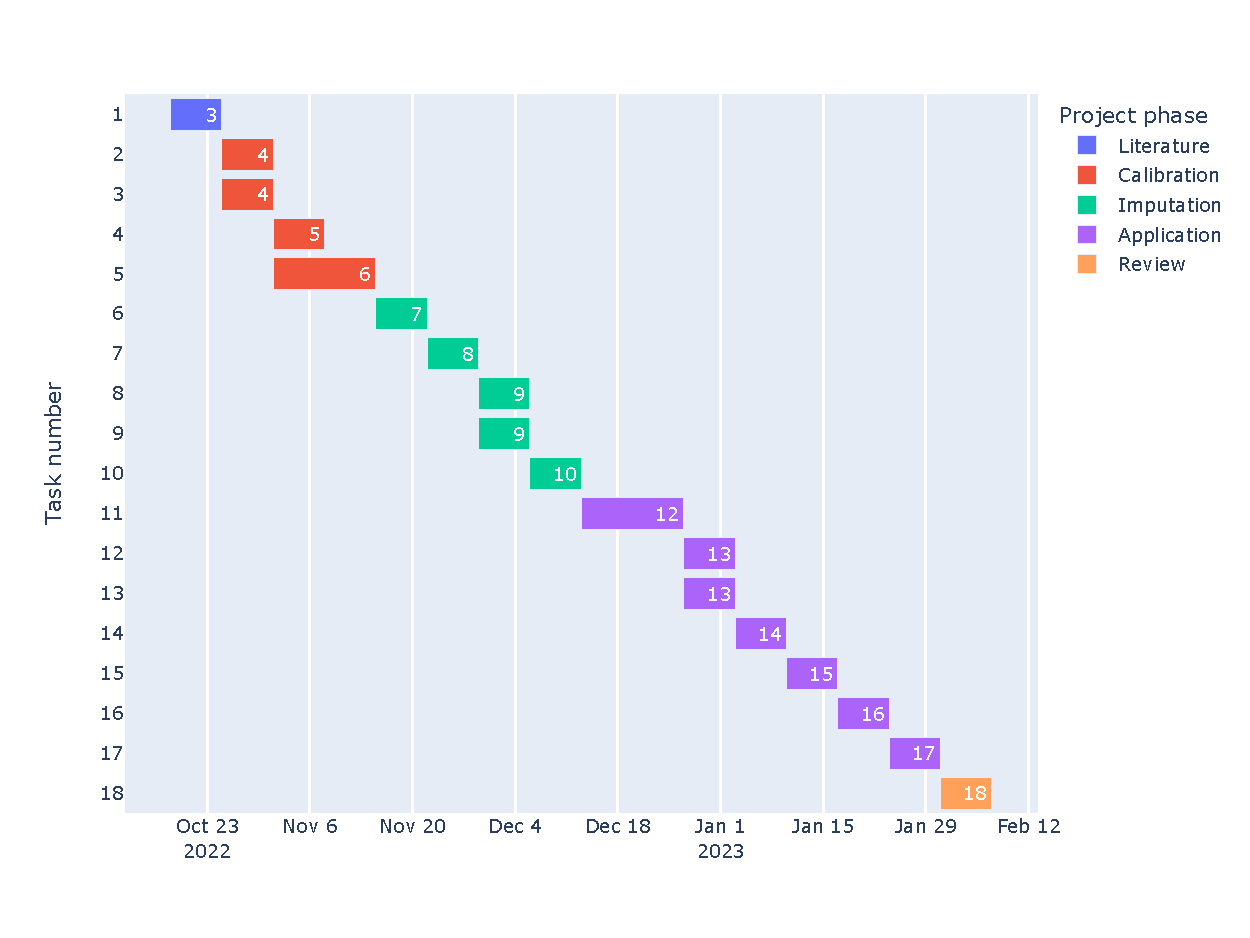
\includegraphics[width=0.5\textwidth]{gantt_chart.pdf}
    \caption{Gantt chart with project milestones}
    \label{gantt_chart}
\end{figure}

\end{document}
